\title{Retrieval and analysis of Eurostat open data with the \pkg{eurostat} package}
\author{Leo Lahti, Janne Huovari, Markus Kainu, Przemys{\l}aw Biecek}

\maketitle

%An abstract of less than 150 words.
\abstract{The increasing availability of open statistical data resources is
providing novel opportunities for research and citizen
science. Efficient algorithmic tools are needed to realize the full
potential of the new information resources. We introduce
the \CRANpkg{eurostat} R package that provides a collection of custom
tools for the Eurostat open data service, including functions to
query, download, manipulate, and visualize these data sets in a
smooth, automated and reproducible manner. The online documentation
provides detailed examples on the analysis of these spatio-temporal
data collections. This work provides substantial improvements over the
previously available tools, and has been extensively tested by an
active user community. The \CRANpkg{eurostat} R package contributes to
the growing open source ecosystem dedicated to reproducible research
in computational social science and digital humanities.}


\section{Introduction}

Eurostat, the statistical office of the European Union, provides a
rich collection of data through its open data
service\footnote{\url{http://ec.europa.eu/eurostat/data/database}},
including thousands of data sets on European demography, economics,
health, infrastructure, traffic and other topics. The statistics are
often available with fine geographical resolution and include time
series spanning over several years or decades.

Availability of algorithmic tools to access and analyse open data
collections can greatly benefit reproducible
research \citep{Gandrud13, Boettiger2015}, as complete analytical
workflows spanning from raw data to final publications can be made
fully replicable and transparent. Dedicated software packages help to
simplify, standardize, and automate analysis workflows, greatly
facilitating reproducibility, code sharing, and efficient data
analytics. The code for data retrieval need to be customized to specific data
sources to accommodate variations in raw data formats, access details,
and typical use cases so that the end users can avoid repetitive
programming tasks and save time. A number of packages for governmental
and other sources have been designed to meet these demands, including
packages for the Food and Agricultural Organization (FAO) of the
United Nations (\CRANpkg{FAOSTAT}; \citealt{FAOSTAT}), World Bank
(\CRANpkg{WDI}; \citealt{WDI}), national statistics authorities
(\CRANpkg{pxweb}; \citealt{pxweb}), Open Street Map
(\CRANpkg{osmar}; \citealt{osmar}) and many other sources.

A dedicated R package for the Eurostat open data has been
missing. The \CRANpkg{eurostat} R package fills this gap. It combines
and expands the capabilities of our earlier \CRANpkg{statfi} \citep{statfi}
and \CRANpkg{smarterpoland} \citep{smarterpoland} packages. Since its
first CRAN release in 2014, the \CRANpkg{eurostat} package has been
actively developed by several contributors via Github based on
frequent feedback from the user community. We are now reporting the
first mature version that has been improved and tested by multiple
users, and applied in several case studies by us and others \citep{Kenett2016}. Eurostat has three services for programmatic data access: a bulk download, json/unicode, and SDMX web service; we provide dedicated methods for the first two data types in the \CRANpkg{eurostat} package; further tools to access SDMX data are available via the generic \CRANpkg{rsdmx} R package \citep{rsdmx}. The bulk download provides single files, which is convenient and fast for retrieving major parts of data. More light-weight json methods allow data subsetting before download and may be preferred in more specific retrieval tasks but the query size is limited to 50
categories. Finally, the package can be used to download custom
administrative boundaries by EuroGeographics\copyright \ that allow
seamless visualization on the Eurostat statistics on the European map.

Certain versions of Eurostat data can be accessed also with the \CRANpkg{datamart} \citep{datamart}, \CRANpkg{quandl} \citep{quandl}, \CRANpkg{pdfetch} \citep{pdfetch}, and \CRANpkg{rsdmx} \citep{rsdmx}
packages. Compared to these generic database packages, \CRANpkg{eurostat}
is particularly tailored for the Eurostat open data service. It
depends on further R packages including
\CRANpkg{classInt} \citep{classInt},
\CRANpkg{dplyr} \citep{dplyr},
\CRANpkg{ggplot2} \citep{ggplot2},
\CRANpkg{httr} \citep{httr},
\CRANpkg{jsonlite} \citep{jsonlite},
\CRANpkg{knitr} \citep{knitr},
\CRANpkg{mapproj} \citep{mapproj}, 
\CRANpkg{RColorBrewer} \citep{RColorBrewer},
\CRANpkg{readr} \citep{readr},
\CRANpkg{sp} \citep{sp},
\CRANpkg{stringi} \citep{stringi},
\CRANpkg{stringr} \citep{stringr}, and
\CRANpkg{tidyr} \citep{tidyr}. The \CRANpkg{eurostat} package is part of the rOpenGov collection
\citep{Lahti13icml} that provides reproducible research tools for
computational social science and digital humanities.

In summary, the \CRANpkg{eurostat} package provides custom tools 
for Eurostat open data. Key features such as cache, date formatting,
tidy data principles \citep{wickham2014},
and \CRANpkg{tibble} \citep{tibble} data format supports seamless
integration with other standard tools for data manipulation and
analysis. This article provides an overview of the core functionality
in the current CRAN release version (2.4.1). A comprehensive
documentation of the package functionality as well as the source code
for this article are available via the package homepage in Github\footnote{http://ropengov.github.io/eurostat}.


\section{Search and download commands}

To install and load the CRAN release version, just type the standard installation command in R.

\begin{example}
> install.packages("eurostat")
> library("eurostat")
\end{example}


The database table of contents is available
on-line\footnote{http://ec.europa.eu/eurostat/data/database}, or can
be downloaded in R with \code{get\_eurostat\_toc()}. A more focused
search is provided by the \code{search\_eurostat()} function.

\begin{example}
> query <- search_eurostat("road accidents", type = "table")
\end{example}

This seeks data on road accidents. The \code{type} argument limits the
search on a selected data set type, one of three hierarchical levels
including \dfn{'table'}, which resides in \dfn{'dataset'}, which is in turn stored in a \dfn{'folder'}. Values in the \code{code} column of the \code{search\_eurostat()} function output provide data identifiers for subsequent download commands. Alternatively, these identifiers can be browsed at the Eurostat open data service; check the codes in the Data Navigation Tree listed after each dataset in parentheses. Let us look at the data identifier and title for the first entry of the query data.

\begin{example}
> query$code[[1]]
[1] "tsdtr420"

> query$title[[1]]
[1] "People killed in road accidents"
\end{example}


Let us next retrieve the data set with this identifier.

\begin{example}
> dat <- get_eurostat(id = "tsdtr420", time_format = "num")
\end{example}

Here we used the numeric time format as it is more convient for annual
time series than the default date format. The transport statistics
returned by this function call (Table~\ref{tab:getdatatable}) could be
filtered before download with the \code{filters} argument, where the
list names and values refer to Eurostat variable and observation
codes, respectively. To retrieve transport statistics for specific
countries, for instance, use the get\_eurostat function.

\begin{example}
> countries <- c("UK", "SK", "FR", "PL", "ES", "PT")
> t1 <- get_eurostat("tsdtr420", filters = list(geo = countries)) 
\end{example}


\begin{table}[ht]
\centering
\begin{tabular}{rlllrr}
\toprule
  \hline
 & unit & sex & geo & time & values \\ 
  \hline
1 & NR & T & AT & 1999.00 & 1079.00 \\ 
  2 & NR & T & BE & 1999.00 & 1397.00 \\ 
  3 & NR & T & CZ & 1999.00 & 1455.00 \\ 
  4 & NR & T & DE & 1999.00 & 7772.00 \\ 
  5 & NR & T & DK & 1999.00 & 514.00 \\ 
  6 & NR & T & EL & 1999.00 & 2116.00 \\ 
   \hline
\bottomrule   
\end{tabular}
\caption{First entries of the road accident data set retrieved with \code{get\_eurostat(id = "tsdtr420", time\_format = "num")}.}
\label{tab:getdatatable}
\end{table}


\begin{table}[ht]
\centering
\begin{tabular}{rlllrr}
\toprule
  \hline
 & unit & sex & geo & time & values \\ 
  \hline
1 & Number & Total & Austria & 1999.00 & 1079.00 \\ 
  2 & Number & Total & Belgium & 1999.00 & 1397.00 \\ 
  3 & Number & Total & Czech Republic & 1999.00 & 1455.00 \\ 
  4 & Number & Total & Germany (until 1990 former territory of the FRG) & 1999.00 & 7772.00 \\ 
  5 & Number & Total & Denmark & 1999.00 & 514.00 \\ 
  6 & Number & Total & Greece & 1999.00 & 2116.00 \\ 
   \hline
\bottomrule      
\end{tabular}
\caption{The \code{get\_eurostat()} output (Table~\ref{tab:getdatatable}) converted into human-readable labels with \code{label\_eurostat()}.}
\label{tab:getdatatable2}
\end{table}



A subsequent visualization reveals a decreasing trend of road accidents over time in Figure~\ref{fig:transport}.

\begin{example}
> ggplot(t1, aes(x = time, y = values, color=geo, group=geo, shape=geo)) +
+   geom_point(size=4) + geom_line() + theme_bw() +
+   ggtitle("Road accidents") + xlab("Year") + ylab("Victims (n)") +
+   theme(legend.position="none") +
+   ggrepel::geom_label_repel(data=t1 %>% group_by(geo) %>% na.omit() %>%
+     filter(time %in% c(min(time), max(time))), aes(fill=geo,label=geo),color="white")
\end{example}

\begin{figure}[h]
\setkeys{Gin}{width=0.5\textwidth, height=0.4\textwidth}
\begin{center}
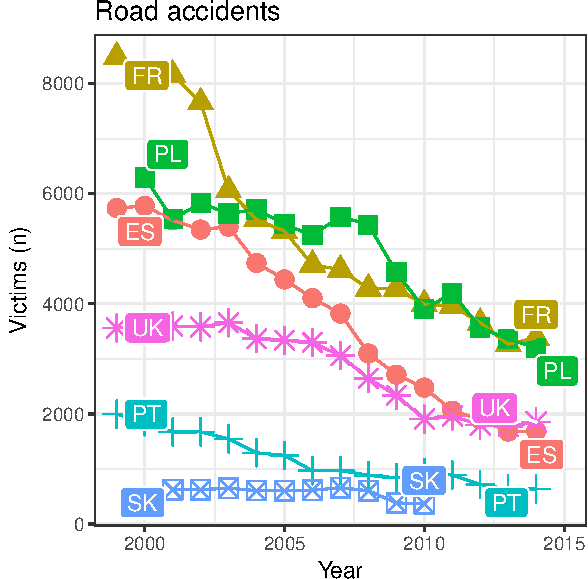
\includegraphics{2015-manu-roadacc-1}
\end{center}
\caption{Timeline indicating the number of people killed in road accidents in various countries based on Eurostat open data retrieved with the \CRANpkg{eurostat} R package.}
\label{fig:transport}
\end{figure}




\section{Utilities}

Many entries in Table~\ref{tab:getdatatable} are not readily interpretable, but a simple call \code{label\_eurostat(dat)} can be used to convert the original identifier codes into human-readable labels (Table~\ref{tab:getdatatable2}) based on translations in the Eurostat database. Labels are available in English, French and German languages.

The Eurostat database includes a variety of demographic and health
indicators. We see, for instance, that overweight varies remarkably
across different age groups (Figure~\ref{fig:bmi}A). Sometimes the
data sets require more complicated pre-processing. Let's consider, for
instance, the distribution of renewable energy sources in different
European countries. In order to summarise such data one needs to first
aggregate a multitude of possible energy sources into a smaller number
of coherent groups. Then one can use standard R tools to process the
data, chop country names, filter countries depending on production
levels, normalize the within country production. After a series of
transformations (see Appendix for the source code) we can finally plot
the data to discover that countries vary a lot in terms of renewable
energy sources (Figure~\ref{fig:bmi}B). Three-dimensional data sets
such as this can be conveniently visualized as triangular maps by
using the \CRANpkg{plotrix} \citep{plotrix} package.

The data sets are stored in cache by default to avoid repeated
downloads of identical data and to speed up the analysis. Storing
an exact copy of the retrieved raw data on the hard disk will also
support reproducibility when the source database is constantly
updated.



\begin{figure}
\setkeys{Gin}{width=0.5\textwidth}
\begin{center}
\begin{tabular}{cc}
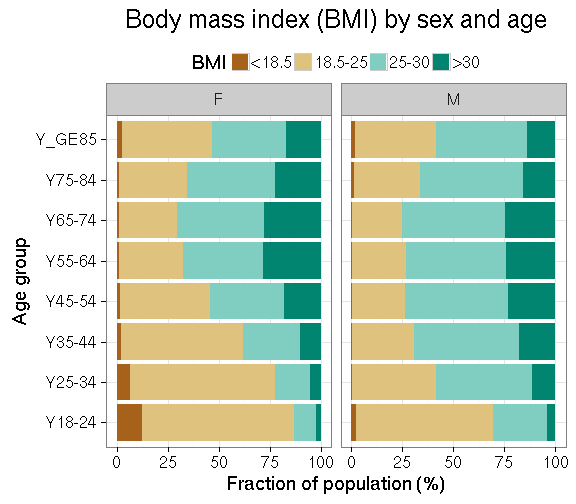
\includegraphics{2015-manu-bmi-1}
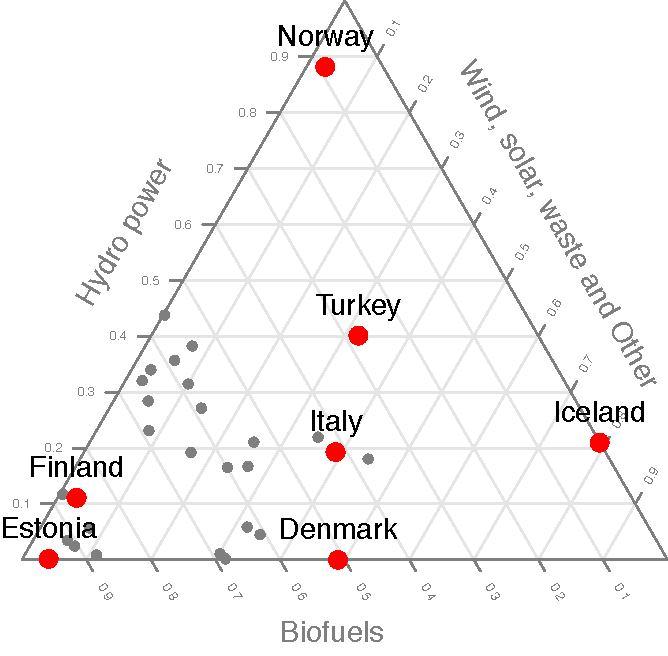
\includegraphics{2015-manu-energy-2}
\end{tabular}
\end{center}
\caption{{\bf A} The body-mass index (BMI) in different age groups in Poland (Eurostat table \texttt{hlth\_ehis\_de1}). {\bf B} Production of renewable energy in various countries in 2013 (Eurostat table \texttt{ten00081}). See the Appendix for the source code.}
\label{fig:bmi}
\end{figure}



\section{Geospatial information}

\subsection{Map visualizations}

The indicators in the Eurostat open data service are typically
available as annual time series grouped by country, and sometimes at
more refined temporal or geographic levels. Eurostat provides
complementary geospatial data on the corresponding administrative
statistical units to support visualizations at the appropriate
geographic resolution. The geospatial data sets are available as
standard
shapefiles\footnote{http://ec.europa.eu/eurostat/web/gisco/geodata/reference-data/administrative-units-statistical-units}. Let
us look at disposable income of private households (data identifier
tgs00026\footnote{http://ec.europa.eu/eurostat/en/web/products-datasets/-/TGS00026}). This
is provided at the geographic NUTS2 regions, the intermediate
territorial units in the Eurostat regional classifications, roughly
corresponding to provinces or states in each
country\footnote{http://ec.europa.eu/eurostat/web/nuts/overview} (Figure~\ref{fig:mapexample}). The map can be generated with the following code chunk.

\begin{example}
> # Loading required libraries
> library(eurostat)
> library(dplyr)
> library(ggplot2)

> # Downloading and manipulating the tabular data
> get_eurostat("tgs00026", time_format = "raw") %>% 
+   # subsetting to year 2005 and NUTS-3 level
+   dplyr::filter(time == 2005, nchar(as.character(geo)) == 4) %>%

+   # Classify the values the variable
+   dplyr::mutate(cat = cut_to_classes(values)) %>%

+   # Merge Eurostat data with geodata from Cisco
+   merge_eurostat_geodata(data = ., geocolumn = "geo", resolution = "60",
+                          output_class = "df", all_regions = TRUE) %>% 

+   # Plot map
+   ggplot(data=., aes(long,lat,group=group)) +
+   geom_polygon(aes(fill = cat),colour=alpha("white", 1/2),size=.2) +
+   scale_fill_manual(values=RColorBrewer::brewer.pal(n = 5, name = "Oranges")) +
+   labs(title="Disposable household income") +
+   coord_map(project="orthographic", xlim=c(-22,34), ylim=c(35,70)) + theme_minimal() +
+   guides(fill = guide_legend(title = "EUR per Year",title.position = "top", title.hjust=0))
\end{example}


This demonstrates how the Eurostat statistics and geospatial data,
retrieved with the eurostat package, can be combined with other
utilities, in this case the
\CRANpkg{grid} \citep{grid}, \CRANpkg{maptools} \citep{maptools}, \CRANpkg{rgdal} \citep{rgdal},
\CRANpkg{rgeos} \citep{rgeos}, \CRANpkg{scales} \citep{scales}, and
\CRANpkg{stringr} \citep{stringr} R packages.

\begin{figure}
\setkeys{Gin}{width=.8\textwidth}
\begin{center}
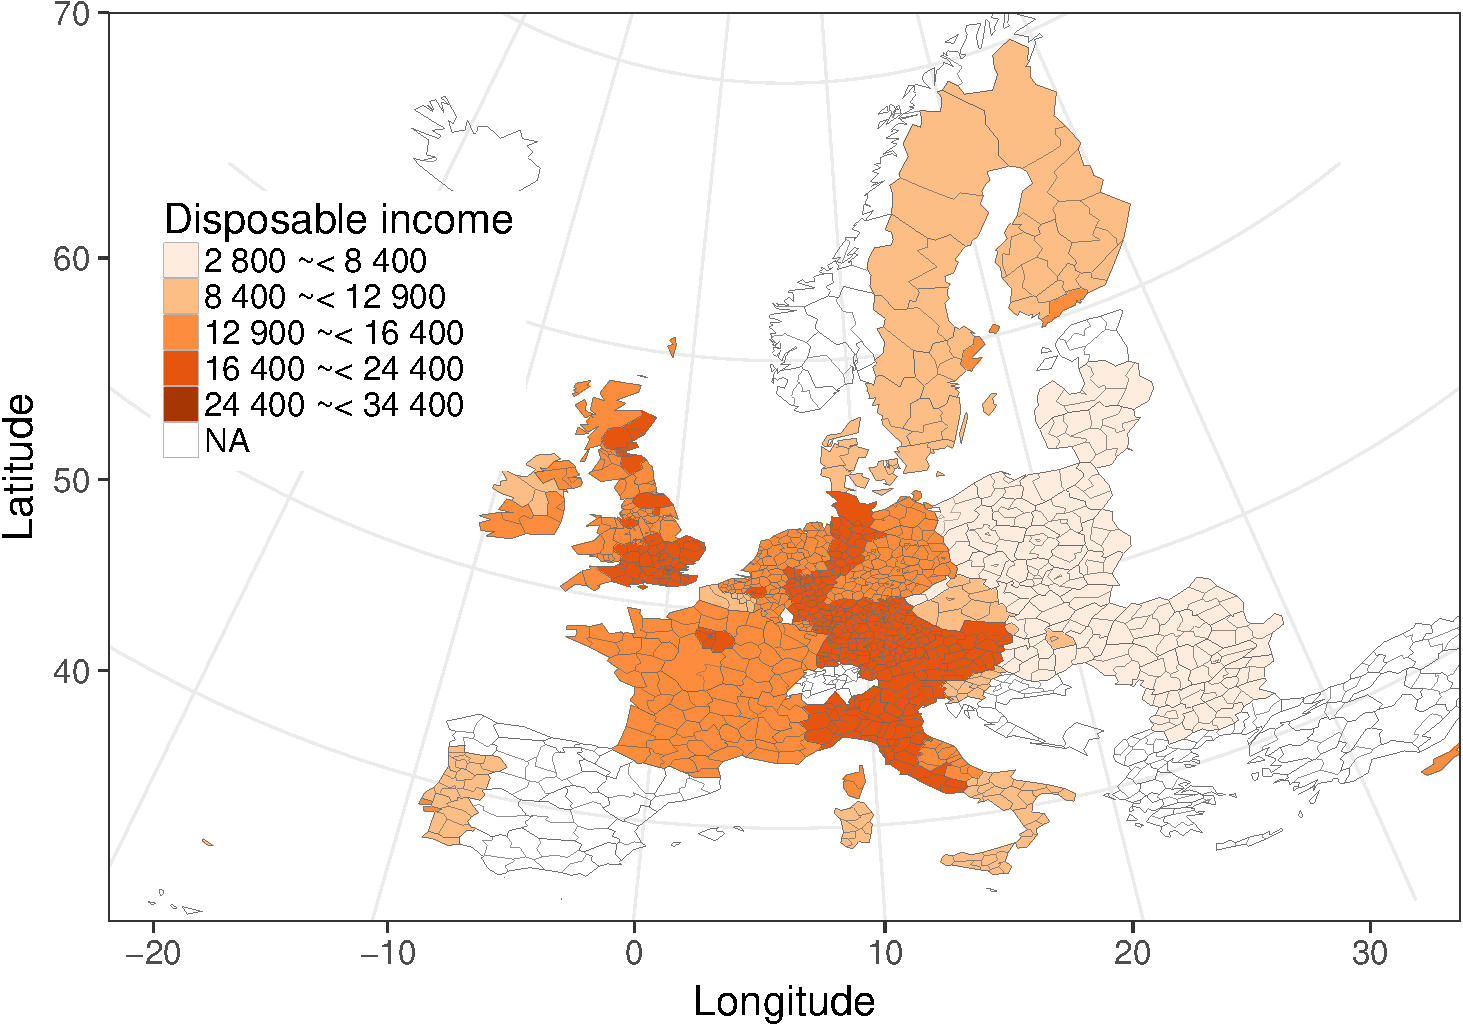
\includegraphics{2015-manu-mapexample-1}
\caption{Disposable income of private households across NUTS2-level national regions in European countries. The household income statistics provided by Eurostat and the administrative boundaries by EuroGeographics\copyright \  were obtained via the Eurostat open data service with the \CRANpkg{eurostat} R package.}
\label{fig:mapexample}
\end{center}
\end{figure}


\subsection{Default country groupings}

To facilitate the analysis and visualization of standard European
country groups, the \CRANpkg{eurostat} package includes ready-made
country code lists. The list of EFTA countries (Table~\ref{tab:efta}),
for instance, is retrieved with the data command.

\begin{example}
> data(efta_countries)
\end{example}

\begin{table}[h]
\centering
\begin{tabular}{rll}
\toprule
  \hline
  & code & name \\ 
  \hline
  1 & IS & Iceland \\ 
  2 & LI & Liechtenstein \\ 
  3 & NO & Norway \\ 
  4 & CH & Switzerland \\ 
   \hline
\bottomrule   
\end{tabular}
\caption{The EFTA country listing from the eurostat R package.}
\label{tab:efta}
\end{table}

Similar lists are available for Euro area (ea\_countries), EU
(eu\_countries) and the EU candidate countries
(eu\_candidate\_countries). These auxiliary data sets facilitate
smooth selection of specific country groups for a closer analysis. The
full name and a two-letter identifier are provided for each country
according to the Eurostat database. The country codes follow the ISO
3166-1 alpha-2 standard, except that GB and GR are replaced by UK
(United Kingdom) and EL (Greece) in the Eurostat database,
respectively. Linking these country codes with external data sets can
be facilitated by conversions between different country coding
standards with the \CRANpkg{countrycode} package \citep{countrycode}.




\section{Discussion}

By combining programmatic access to data with custom analysis and visualization tools it is possible to facilitate a seamless automation of the complete analytical workflow from raw data to statistical summaries and final publication. The package supports automated and transparent data retrieval from institutional data repositories, featuring options such as search, subsetting and cache. Moreover, it provides several custom functions to facilitate the Eurostat open data analysis and visualization. These tools can be readily used by researchers and statisticians in academia, government, and industry, and their applicability has been demonstrated in recent, independent publications \citep{Kenett2016}. 

The \CRANpkg{eurostat} R package provides a convenient set of tools to access open data from Eurostat, together with a comprehensive documentation and open source code via the package homepage\footnote{http://ropengov.github.io/eurostat}. The documentation includes simple examples for individual functions, a generic package tutorial, and more advanced case studies on data processing and visualization. The package follows best practices in open source software development, taking advantage of version control, automated unit tests, continuous integration, and collaborative development model \citep{PerezRiverol2016}.

The package source code can be freely used, modified and distributed under a modified BSD-2-clause license\footnote{https://opensource.org/licenses/BSD-2-Clause}. We value feedback from the user community, and the package has already benefited greatly from the user bug reports and feature requests, which can be systematically provided through the Github issue tracker\footnote{https://github.com/rOpenGov/eurostat/issues}; advanced users can also implement and contribute new features by making pull requests. Indeed, we have already accommodated a number of proposed changes and accepted multiple pull requests during the package development. We are committed to active maintenance and development of the package, and hope that this will encourage further feedback and contributions from the user community.


\section*{Acknowledgements}

We are grateful to all package contributors, including Joona
Lehtom{\"a}ki, Oliver Reiter and Fran\c{c}ois Briatte and to Eurostat
for maintaining the open data service. This work is in no way
officially related to or endorsed by Eurostat. The work has been
partially funded by Academy of Finland (decisions 295741, 307127), and
part of the rOpenGov\footnote{https://github.ropengov.io} project.


\bibliography{lahti-huovari-kainu-biecek}

\address{Leo Lahti\\
  Department of Mathematics and Statistics\\
  PO Box 20014 University of Turku\\
  Finland\\}
\email{leo.lahti@iki.fi}

\address{Janne Huovari\\
  Pellervo Economic Research PTT\\
  Eerikinkatu 28 A 00180 Helsinki\\
  Finland\\}
\email{janne.huovari@ptt.fi}

\address{Markus Kainu\\
  Research Department, The Social Insurance Institution of Finland\\
  PO Box 450, 00101 Helsinki\\
  Finland\\}
\email{markus.kainu@kela.fi}

\address{Przemys{\l}aw Biecek\\
  Faculty of Mathematics and Information Science\\
  Warsaw University of Technology\\
  Koszykowa 75, 00-662 Warsaw\\
  Poland\\}
\email{P.Biecek@mimuw.edu.pl}

\newpage

\section{Appendix}

The full reproducible source code for the examples from this manuscript is provided at the package homepage\footnote{http://ropengov.github.io/eurostat}. Source code for the obesity example (Figure~\ref{fig:bmi}A) is as follows.

\begin{example}
> library(dplyr)
> tmp1 <- get_eurostat("hlth_ehis_de1", time_format = "raw")
> tmp1 %>%
+  dplyr::filter( isced97 == "TOTAL" ,
+          sex != "T",
+          age != "TOTAL", geo == "PL") %>%
+  mutate(BMI = factor(bmi, 
+                      levels=c("LT18P5","18P5-25","25-30","GE30"), 
+                      labels=c("<18.5", "18.5-25", "25-30",">30"))) %>%
+  arrange(BMI) %>%
+  ggplot(aes(y=values, x=age, fill=BMI)) + geom_bar(stat="identity") +
+  facet_wrap(~sex) + coord_flip() +
+  theme(legend.position="top") +
+  ggtitle("Body mass index (BMI) by sex and age") +
+  xlab("% of population") + scale_fill_brewer(type = "div")
\end{example}


Source code for the renewable energy example (Figure~\ref{fig:bmi}B).

\begin{example}
# All sources of renewable energy are to be grouped into three sets
> dict <- c("Solid biofuels (excluding charcoal)" = "Biofuels",
+          "Biogasoline" = "Biofuels",
+          "Other liquid biofuels" = "Biofuels",
+          "Biodiesels" = "Biofuels",
+          "Biogas" = "Biofuels",
+          "Hydro power" = "Hydro power",
+          "Tide, Wave and Ocean" = "Hydro power",
+          "Solar thermal" = "Wind, solar, waste and Other",
+          "Geothermal Energy" = "Wind, solar, waste and Other",
+          "Solar photovoltaic" = "Wind, solar, waste and Other",
+          "Municipal waste (renewable)" = "Wind, solar, waste and Other",
+          "Wind power" = "Wind, solar, waste and Other",
+          "Bio jet kerosene" = "Wind, solar, waste and Other")
# Some cleaning of the data is required
> energy3 <- get_eurostat("ten00081") %>%
+  label_eurostat(dat) %>% 
+  filter(time == "2013-01-01",
+         product != "Renewable energies") %>%
+  mutate(nproduct = dict[as.character(product)], # just three categories
+         geo = gsub(geo, pattern=" \\(.*", replacement="")) %>%
+  select(nproduct, geo, values) %>% 
+  group_by(nproduct, geo) %>%
+  summarise(svalue = sum(values)) %>%
+  group_by(geo) %>%
+  mutate(tvalue = sum(svalue),
+         svalue = svalue/sum(svalue)) %>%
+ filter(tvalue > 1000) %>% 
+ spread(nproduct, svalue)
+ # Triangle plot
+ positions <- plotrix::triax.plot(as.matrix(energy3[, c(3,5,4)]),
+           show.grid = TRUE, label.points= FALSE, point.labels = energy3$geo,
+          col.axis="gray50", col.grid="gray90",
+          pch = 19, cex.axis=1.1, cex.ticks=0.7, col="grey50")
+ ind <- which(energy3$geo %in%  c("Norway", "Iceland","Denmark","Estonia", "Turkey", 
+          "Italy", "Finland"))
+ df <- data.frame(positions$xypos, geo = energy3$geo)
+ points(df$x[ind], df$y[ind], cex=2, col="red", pch=19)
+ text(df$x[ind], df$y[ind], df$geo[ind], adj = c(0.5,-1), cex=1.5)
\end{example}




